%% Template for English Papers
%%%%%%%%%%%%%%%%%%%%%%%%%%%%%%%%%%%%%%%%%%%%%%%%%%%%%%%%%%%%%%%%%%%%%%%%%%%%%%%
 \documentclass[english]{jpnsecart}                   % English Original Paper

%% For JPNSEC office %%%%%%%%%%%%%%%%%%%%%%%%%%%%%%%%%%%%%%%%%%%%%%%%%%%%%%%%%%
% You don't need to modify them. 
\received{2010}{8}{1}
\stuffincharge{XX\hspace{0.5zh} XX}
\setcounter{page}{1}
%\setcounter{volpage}{1}
\Vol{1}
\No{1}

%% CAUSION for amsmath package users %%%%%%%%%%%%%%%%%%%%%%%%%%%%%%%%%%%%%%%%%%
% \usepackpage{amsmath}
% equation No. should be reffered by the \eqref, not \ref
% specify the "fleqn" as the option of documentclass command
% ex. \documentclass[technicalpaper,fleqn]{jpnsecart}
%\usepackage{evocomp}
\usepackage{fancyhdr}
\usepackage{graphicx}
%\addcontentsline{toc}{chapter}{Bibliography}
\usepackage{amsmath}
\usepackage{amssymb}
\usepackage{algorithm}
\usepackage[noend]{algpseudocode}
\usepackage{booktabs}

\usepackage{colortbl}

\newcommand{\gray}{\rowcolor[gray]{.90}}


%% Title %%%%%%%%%%%%%%%%%%%%%%%%%%%%%%%%%%%%%%%%%%%%%%%%%%%%%%%%%%%%%%%%%%%%%%
\etitle{MOEA/D-RAD - Resource Allocation by Diversity}
% \etitle[English Title for Headers]{English Title}
%\esubtitle{Resource Allocation by Diversity}

%% Authors %%%%%%%%%%%%%%%%%%%%%%%%%%%%%%%%%%%%%%%%%%%%%%%%%%%%%%%%%%%%%%%%%%%%
% when authers whose affilication is the same is succeed, 
% use \affiliation macro for the top of the succeed authers 
% and use \sameaffiliation for the rest of the authors.
% Delete the following line if the number of author is less than four.
\manyauthor 
\author{%
 \name{Yuri}{Lavinas}
 \affiliation{University of Tsukuba, Graduate School of Systems and Information Engineering, Japan}%
     {yclavinas@gmail.com}
\and
 \name{Claus}{Aranha}
  \sameaffiliation{caranha@cs.tsukuba.ac.jp}
\and
 \name{Tetsuya}{Sakurai}
 \sameaffiliation{sakurai@cs.tsukuba.ac.jp}
}

%% Keywords, Summary %%%%%%%%%%%%%%%%%%%%%%%%%%%%%%%%%%%%%%%%%%%%%%%%%%%%%%%%%%
\begin{keyword}
	Resource Allocation, Diversity assessment, Multiobjective Optimization, Priority Functions.
\end{keyword}

\begin{summary}
	MOEA/D decomposes multi-objective problems into single-objective subproblems and solve them in parallel. In standard MOEA/D, all subproblems receive the same computational effort. However, as each subproblem is related to a different area of the objective space, it is expected that some subproblems are more difficult than others. Using Resource Allocation, MOEA/D could spend less effort on easier subproblems and more on harder ones, improving efficiency. In this paper, we address Resource Allocation that uses priority functions. They determine which subproblems should receive more computation resources. We propose the MOEA/D-RAD, a MOEA/D that considers diversity in the decision space as the measure of priority among candidate solutions. We compare MOEA/D-RAD, MOEA/D-DE and MOEA/D-DRA on the bbob-biobj benchmark, composed of 55 functions grouped into 15 groups, based on the function properties. We investigate the performance of these three methods based on hypervolume and proportion of non-dominated solutions in all of these 15 groups. Exploratory experiments show that MOEA/D-RAD obtained the best hypervolume in 24 functions. In particular MOEA/D-RAD obtained a good performance in groups characterized by moderated and weakly-structured groups.These results validate the effectiveness of using diversity in the objective space as priority function in the MOEA/D framework.
\end{summary}

%% Body %%%%%%%%%%%%%%%%%%%%%%%%%%%%%%%%%%%%%%%%%%%%%%%%%%%%%%%%%%%%%%%%%%%%%%%
\begin{document}
\maketitle

\input{1_intro_copy.tex}
\section{Related Works}

\subsection{Priority functions}

%Following the discussion opened in the introduction, we need to define an utility function to allocate the number of evaluations to subproblems. 
We define priority functions (also called utility functions) as one way of establishing preferences between solutions for Resource Allocation~\cite{chankong1983multiobjective}. These functions are used to decide how to allocate computational resources among subproblems by monitoring the algorithm search and guiding the distribution over iterations~\cite{cai2015external}. 

Only a few studies have been concerned with Resource Allocation in MOEA/D. We highlight two groups. The first is composed by MOEA/D-GRA~\cite{zhou2016all}, MOEA/D-DRA~\cite{zhang2009performance} and in the Two-Level Stable Matching-Based Selection in MOEA/D~\cite{nasir2011improved}. The other is composed by EAG-MOEA/D~\cite{cai2015external} and MOEA/D-CRA~\cite{kang2018collaborative}.

According to Zhou and Zhang~\cite{zhou2016all}, MOEA/D-GRA could be seen as an extension of MOEA/D-DRA and MOEA/D-AMS~\cite{chiang2011moea}. They reason that all these algorithms use a very similar priority function and that MOEA/D-GRA can simulate the behavior of MOEA/D-DRA or MOEA/D-AMS by changing the values of a single parameter. 

This priority function is named as the Relative Improvement (R.I.) and defines the priority values of each subproblem $i=1,...,N$, as

\begin{equation}\label{priority}
\delta_i = \dfrac{\text{old function value}-\text{new function value}}{\text{old function value}}.
\end{equation}

Where new function value is the value at the current iteration ($T$) and old function value is the value at iteration ($T - \Delta T$).

For MOEA/D-GRA $u_i = \delta_i$, but in MOEA/D-DRA, as well as in the Two-Level Stable Matching-Based Selection in MOEA/D, a second equation is used,

\[
u_i= 
\begin{cases}

(0.95 + 0.05 \cdot \frac{\delta_i}{0.001} \cdot u_i), & \text{if } \delta_i > 0.001,
\\
1,              & \text{otherwise}

\end{cases}\label{priority2}
\]
The R.I. is based the assumption that if a subproblem has been improved over the last $\Delta T$ iteration (\textit{old function value}), it should have a high probability of being improved over the next iterations. 

The priority function used EAG-MOEA/D~\cite{cai2015external} and MOEA/D-CRA~\cite{kang2018collaborative} differ from the ones in the MOEA/D-GRA group. In their case, the framework keeps two populations: one working population, and one external archive. This priority function estimates priorities for a subproblem given the number of solutions from that subproblem that are in the external archive.

Together these studies indicate that it is worth monitoring the algorithm behavior and guiding its search, but it is unclear how the choice of priority functions influence the results. In all Resource Allocation works mentioned above, the choice of priority function was just one of multiple changes applied to the base framework. For example, in Zhang et al. used a 10-tournament selection in MOEA/D-DRA~\cite{zhang2009performance}, while Zhou and Zhang used a new replacement strategy in MOEA/D-GRA~\cite{zhou2016all}. Chiang in MOEA/D-AMS proposes an adaptive mating selection mechanism as it dynamically adjusts the mating pools of individuals~\cite{chiang2011moea}. Finally, both the studies of Cai and Lai in  EAG-MOEA/D~\cite{cai2015external} and Kang et al. in MOEA/D-CRA~\cite{kang2018collaborative} used an archive population.

We focus on improving the performance of the standard MOEA/D by using priority functions, given the recent success of addressing Resource Allocation with priority functions. We believe in the idea that diversity is a critical issue in the search process for any multi-objective algorithm. Therefore, we consider using priority functions to address lack of diversity aiming to make solutions better spread among each other. The proposed priority function focus on how to better spread solutions the Pareto Set (diversity on the decision space). For that, we define the MRDL priority function.



\subsection{Diversity Metric}


One way to measure diversity is to use metrics that evaluate MOPs solvers. The hypervolume indicator (HV)~\cite{zitzler1998multiobjective} and the Inverted Generational Distance (IGD)~\cite{zhang2008rm} are frequently used as metrics to evaluate such solvers. However they include information about both quality of the solutions and diversity in a single metric.

Among the metrics that only measure diversity, there are mainly two groups. The offline group, that calculate the diversity after the execution of the algorithm, while online group, that calculate the diversity during the execution of the algorithm. We are interested in measuring diversity during the execution of the algorithm, therefore we  briefly introduce some studies that are part of the online group.
%
% The offline group is composed of: Chi-square-like deviation~\cite{deb1989genetic}; Spacing method~\cite{scott1995fault}; Uniformly distribution index~\cite{tan2002evolutionary}; Entropy approach~\cite{farhang2002diversity}; Grid diversity metric~\cite{deb2002running}; sparsity measure~\cite{deb2003fast}. These published studies need knowledge of the PF or the ideal vector. While the online group is composed of: sigma method~\cite{mostaghim2003strategies}  (PF lies in the positive objective space); entropy of the solutions by using Parzen window density estimation-\cite{tan2008evolutionary} (sensitive to kernel width); maximum relative diversity loss~\cite{gee2015online} (expensive $O(N^2)$, with $N$ being the size of the parent population).

The online group includes: sigma method~\cite{mostaghim2003strategies}  (PF lies in the positive objective space); entropy of the solutions by using Parzen window density estimation-\cite{tan2008evolutionary} (sensitive to kernel width); and maximum relative diversity loss, MRDL, ~\cite{gee2015online} (expensive $O(N^2)$, with $N$ being the size of the parent population).



In this work we chose to apply the MRDL as the strategy to measure diversity on the objective space. This is an online diversity metric estimates the diversity loss of a solution to the whole population~\cite{gee2015online}. High values indicate the existence of similar solutions or that the offspring solution is close to the convergence direction. The further an objective vector of a solution is from the convergence direction, the more it contributes for the diversity of the approximated the Pareto Front. The MRDL is the maximum value for Relative Diversity Loss (RDL) of each solution.




\section{Proposed Method}
In this work we propose a variant of the MOEA/D, the MOEA/D with online Resource Allocation by Diversity Metric (MOEA/D-RAD). This algorithm uses the maximum relative diversity loss, MRDL, for determining the values of the priority function. 


\begin{algorithm}[h]
	\caption{MOEA/D-RAD}\label{alg1}
	\begin{algorithmic}[1]
		
		\State Initialize the weight vectors $\lambda_i$, the neighborhood $B_i$, the priority value $u_i$ every subproblem $i=1,...,N$.
		
		\While{\textit{Termination criteria}}
		\For {1 to N}
		\If{$\textit{rand()} < u_i$}
		\State Generate an offspring $y$ for subproblem $i$.
		\State Update the population by $y$.
		\EndIf
		\EndFor
		\State  Evaluate and after $\Delta T$ iterations, keep updating \textit{\textbf{u}} by a priority function.
		\EndWhile
	\end{algorithmic}
	%\vspace{-1em}
\end{algorithm}

MOEA/D-RAD is described in algorithm~\ref{alg1}. This basic algorithm is similar to the MOEA/D-DE~\cite{zhang2009performance} with exception of lines 4 and 7. Line 4 deals with the selection of solutions given their priority function values, while the line 7 deals with the calculation of the priority function values. All other procedures and parameters are the same as in MOEA/D-DE~\cite{li2009multiobjective}. We highlight that the neighborhood is only calculated in the initialization period.

%\subsection{Priority Functions}

The selection of priority functions provides an important way to control MOEA/D. They allow ways of designing MOEA/D variants that might focus on desired characteristics, such as diversity, performance contribution, convergence to a specific region of the PF or others. This is possible because different methods can be used as priority functions to create the vector $u$ in algorithm~\ref{alg1}. 

We initialize the value of the vector $u=1$, as in MOEA/D-DRA. As in DRA and GRA we have a learning period of $\Delta T$ iterations. Here $\Delta T=20$ as in MOEA/D-GRA~\cite{zhou2016all}. A sensitivity analysis should be performed for deciding suitable initial values for $u$ and for $\Delta T$.

 It should also be noted that if the priority function values results in less than 3 subproblems being updated in one iteration, we reset the priority vector $u = 1$  and all subproblems will be chosen for offspring reproduction at the that iteration.


\subsection{Priority Function - MRDL} 


\begin{algorithm}[t]
	\caption{MRDL}\label{alg2}
	\begin{algorithmic}[1]
		
		\State Input: old MRDL (initial value is 0); $Y^t$, objective function values from the incumbent solutions; $Y^{t-1}$, objective function values from the incumbent solutions of the previous iteraction; N, the population size.		
		\For {i=1 to N}
		\State find index $h$ where  ($Y^{t-1}_h \succeq Y^t_i$) and $||Y^{t-1}_h - Y^t_i  ||$ is minimal.
		\If {If none is found} 
		\State MRDL[i] = $-\infty$
		\Else
		\State $d.conv = Y^t_i - Y^{t-1}_h$.
		\For {j=1 to N}
		\State $p \prime = Y^{t-1}_j - Y^{t-1}_h$
		\State $c \prime = Y^t_j - Y^t_i$
		\State $proj_{d.conv}*p \prime = \dfrac{sum(conv \cdot p \prime)}{(p \prime \times p \prime)}*p \prime$
		
		\State $ proj_{d.conv}*c \prime = \dfrac{sum(conv \cdot c \prime)}{(c \prime \times c \prime)}*c \prime$
		
		\State $RDL_j = \dfrac{ ||p \prime - proj_{d.conv}p \prime|| }{||c \prime - proj_{d.conv}c \prime||}$\\
		
		\EndFor
		MRDL[i] = maximum $RDL$
		\EndIf
		\EndFor
		\State u = 1 - scale (MRDL - old MRDL) // between 0 and 1\\
	\Return u, MRDL
	\end{algorithmic}
\end{algorithm}

To consider diversity on the objective space, we propose a priority function based on the the Maximum Relative Diversity Loss, MRDL~\cite{gee2015online}.


The diversity on objective space as a priority function  is based on the Maximum Relative Diversity Loss, MRDL~\cite{gee2015online}.  The idea of using MRDL is that by measuring diversity on the objective space, more resources are given to incumbent solutions that have similar objective function values between two consecutive iteractions. Therefore, it is expected that this will lead to a higher exploration of the objective space. Algorithm~\ref{alg2} gives the details on implementation.

The calculation of MRDL depends on the concept of weak dominance~\cite{zitzler2003performance}. A solution $a$ weakly dominates $b$ if in all objectives $a \geq b$ (note that $a \succeq a$).
 
Let $N$ be the number of incumbent solutions and the objective values of iteraction $t$ be $Y^t$ and the objectives values of iteraction $t-1$ be $Y^{t-1}$. For each incumbent solution $i$, find index $h \in Y^{T-1}$. This index is the index of a parent that weak dominates the solution $i$. If $h$ is not found (no parent weak dominates the solution) the MRDL value for this solution is set to $-\infty$. Given $i$ and $h$, for each subproblem, the value of Relative Diversity Loss (RDL) is given by 

\begin{equation}
RDL = \dfrac{ ||p \prime - proj_{d.conv}p \prime|| }{||c \prime - proj_{d.conv}c \prime||}.
\end{equation}


RDL is a diversity measurement quantity that indicates the amount of diversity loss of an individual solution between two consecutive iterations. High values of RDL imply a reduction of the solution spread, since the further an objective vector of a solution is from the convergence direction, the more it contributes in terms of diversity in the objective space~\cite{gee2015online}. The maximum value of RDL is the MRDL of the solution $i$.



\section{Experimental Design}

%\begin{table}[!t]
%	\centering
%\begin{tabular}{@{}|l|l|@{}}
%		\toprule
%		\textbf{Parameters}   & \textbf{Values}          \\ \midrule
%		Initial value $u$     & 0.5, for every subproblem \\ 
%		Population size       & 150                      \\
%		Neighborhood size T & 20 \\ 
%		$\delta_p$ & 0.9 \\ 
%		$\phi$ & 0.5 \\ 
%		$\eta_m$ & 20 \\
%		$p_m$ & 0.03333333 \\
%		$n_r$ & 2 \\
%		\midrule
%		Number of evaluations & 60000 		\\		
%		Number of repetitions & 21                  \\ \bottomrule
%
%	\end{tabular}
%\vspace{1em}
%\caption{Parameter settings.}
%\label{table1}
%\end{table}

To examine the effects of MOEA/D-RAD we perform a comparative experiment of BiBBOB benchmark functions. In this experiment, we use the MOEA/D-DE implemented by the MOEADr package~\cite{moeadr_package}, modified to include Resource Allocation as described in the previous section. We compare three different algorithms MOEA/D-DE and MOEA/D-DRA as well as the proposed MOEA/D-RAD.

\subsection{Target Problems}\label{target_problems}

The Black-Box Optimization Bi-Objective Benchmark (bbob-biobj) test functions~\cite{tusar2016coco} are used as our benchmark problem sets. This test suit is composed of 55 bi-objective functions combined into 15 different classes.

We list below the function classes:

\begin{itemize}
	\item Group 1: separable - separable;% ($f_1, f_2, f_{11}$)
    \item Group 2: separable - moderate;% ($f_3, f_4, f_{12}, f_{13}$)
	\item Group 3: separable - ill-conditioned;% ($f_5, f_6, f_{14}, f_{15}$)
	\item Group 4: separable - multi-modal;% ($f_7, f_8, f_{16}, f_{17}$)
	\item Group 5: separable - weakly-structured;% ($f_9, f_{10}, f_{18}, f_{19}$)
	\item Group 6: moderate - moderate;% ($f_{20}, f_{21}, f_{28}$)
	\item Group 7: moderate - ill-conditioned;% ($f_{22}, f_{23}, f_{29}, f_{30}$)
	\item Group 8: moderate - multi-modal;% ($f_{24}, f_{25}, f_{31}, f_{32}$)
	\item Group 9: moderate - weakly-structured;% ($f_{26}, f_{27}, f_{33}, f_{34}$)
	\item Group 10: ill-conditioned - ill-conditioned;% ($f_{35}, f_{36}, f_{41}$)
	\item Group 11: ill-conditioned - multi-modal;% ($f_{37}, f_{38}, f_{42}, f_{43}$)
	\item Group 12: ill-conditioned - weakly-structured;% ($f_{39}, f_{40}, f_{44}, f_{45}$)
	\item Group 13: multi-modal - multi-modal;% ($f_{46}, f_{47}, f_{50}$)
	\item Group 14: multi-modal - weakly structured;% ($f_{48}, f_{49}, f_{51}, f_{52}$)
	\item Group 15: weakly-structured - weakly-structured.% ($f_{53}, f_{54}, f_{55}$)
\end{itemize}

Here we give a simple explanation of the classes. A separable function does not show any dependencies between the variables while a multi-modal function have at least two minima. Moderate- and ill-conditioned have a high sensitivity in the contribution of a solution to the objective function value~\cite{hansen2011impacts}. Finally, a weakly-structured function is a function that the general structure is very unclear~\cite{finck2010real}.


\subsection{Experimental Parameters}

We use the conventional MOEA/D-DE parameters~\cite{li2009multiobjective} for each Resource Allocation strategy: update size $nr = 2$, neighborhood size $T = 20$, and the neighborhood search probability $\delta_p = 0.9$. The DE mutation operator value is $phi=0.5$. The Polynomial mutation operator values are $\eta_m 20$ and $p_m = 0.03333333$. The decomposition function is Simple-Lattice Design (SLD), the scalar aggregation function is Weighted Sum (WS), the update strategy is the Restricted Update Strategy and we performed a simple linear scaling of the objectives to [0, 1].

For every strategy/function pair we perform 21 repetitions with 30000 function evaluations and population size $N=150$.

\subsection{Experimental Evaluation}

We compare the results of the different strategies based on their Hypervolume (HV) metric. Higher values of the HV indicate better approximations of the Pareto Front. % We also evaluate the proportion of non-dominated solutions and the number of feasible solutions.

For the calculation of HV, the objective function was scaled to the $0,1$ interval, and the reference point was set to $(1,1)$. To verify any statistical differences in the results for the different strategies, we use the Pairwise Wilcoxon Rank Sum Tests with confidence interval $\alpha = 0.05$ and with the Hommel adjustment method for multiple comparisons. %For reproducibility purposes, all the code and data used in these experiments are available at [ANONYMIZED].

\section{Results}



\begin{figure*}[!t]
	\centering
	%	\Large{Average performance on different tournament size - Gallagher's Gaussian 21-hi Peaks Function}
	\begin{subfigure}[b]{0.33\textwidth}
		\centering
		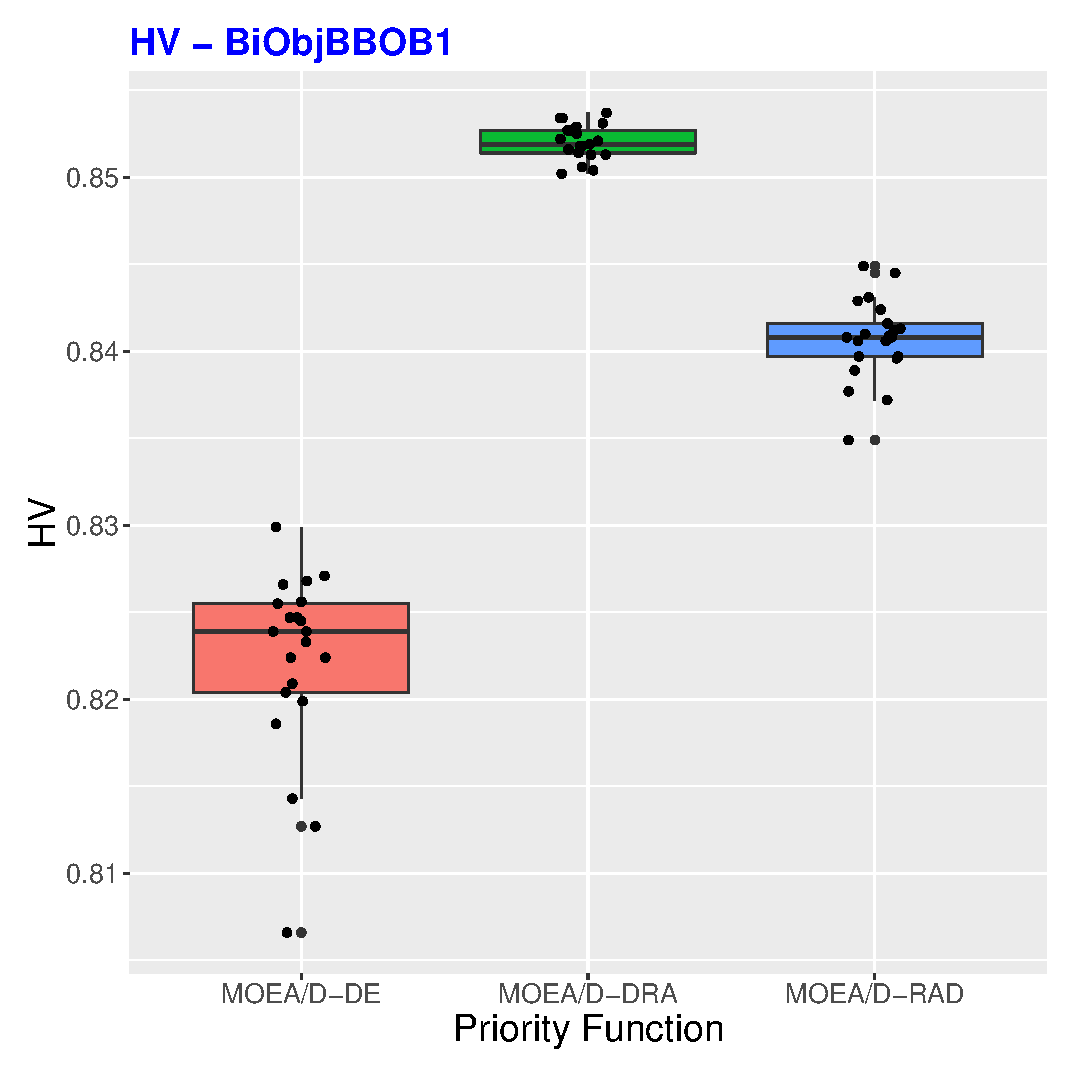
\includegraphics[width=1\textwidth, height=1\textwidth]{img/BiObjBBOB1_HV.eps}
		%	\caption{HV - UF3}
	\end{subfigure}
	\begin{subfigure}[b]{0.33\textwidth}
		\centering
		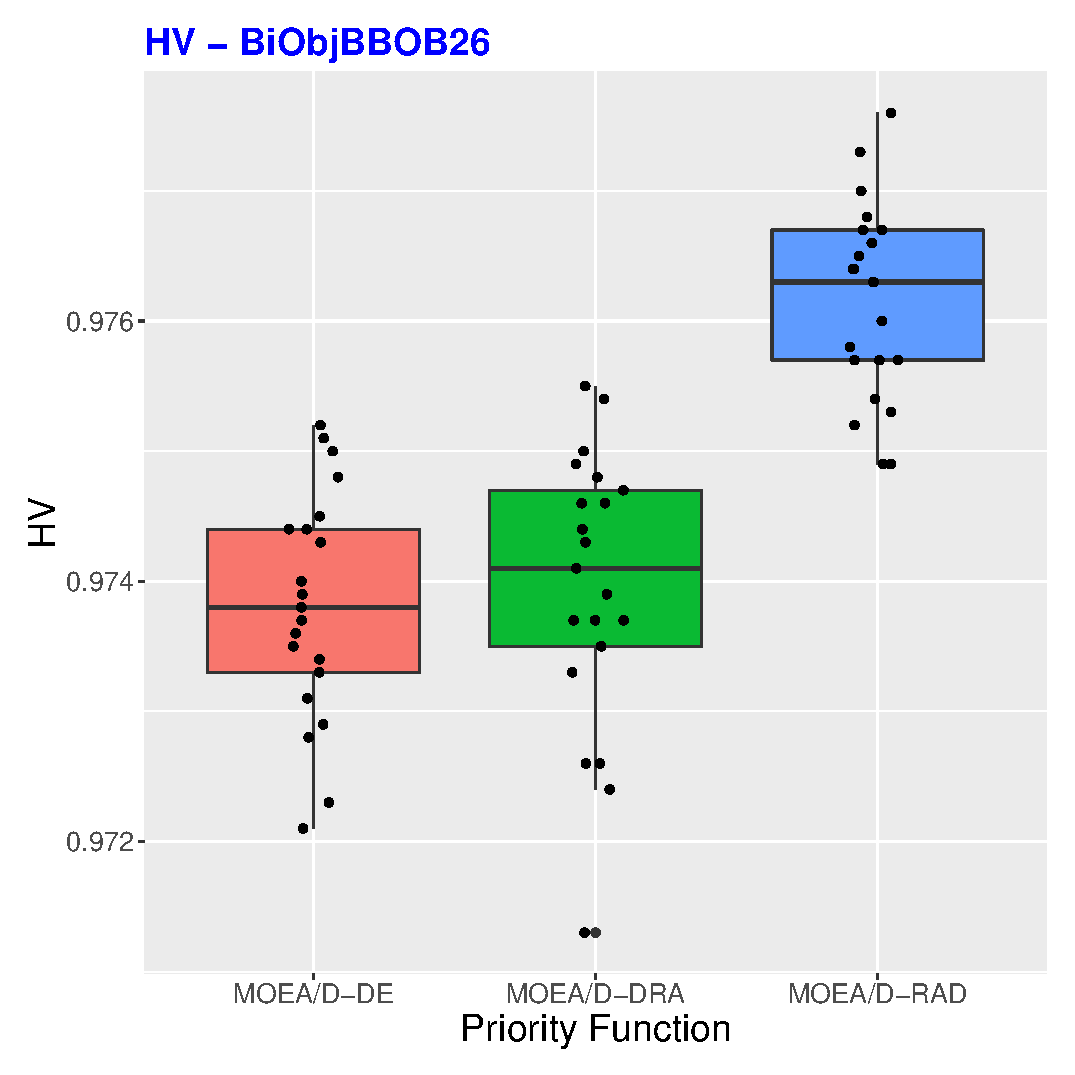
\includegraphics[width=1\textwidth, height=1\textwidth]{img/BiObjBBOB26_HV.eps}
		%	\caption{HV - UF8}
	\end{subfigure}
	\begin{subfigure}[b]{0.33\textwidth}
		\centering
		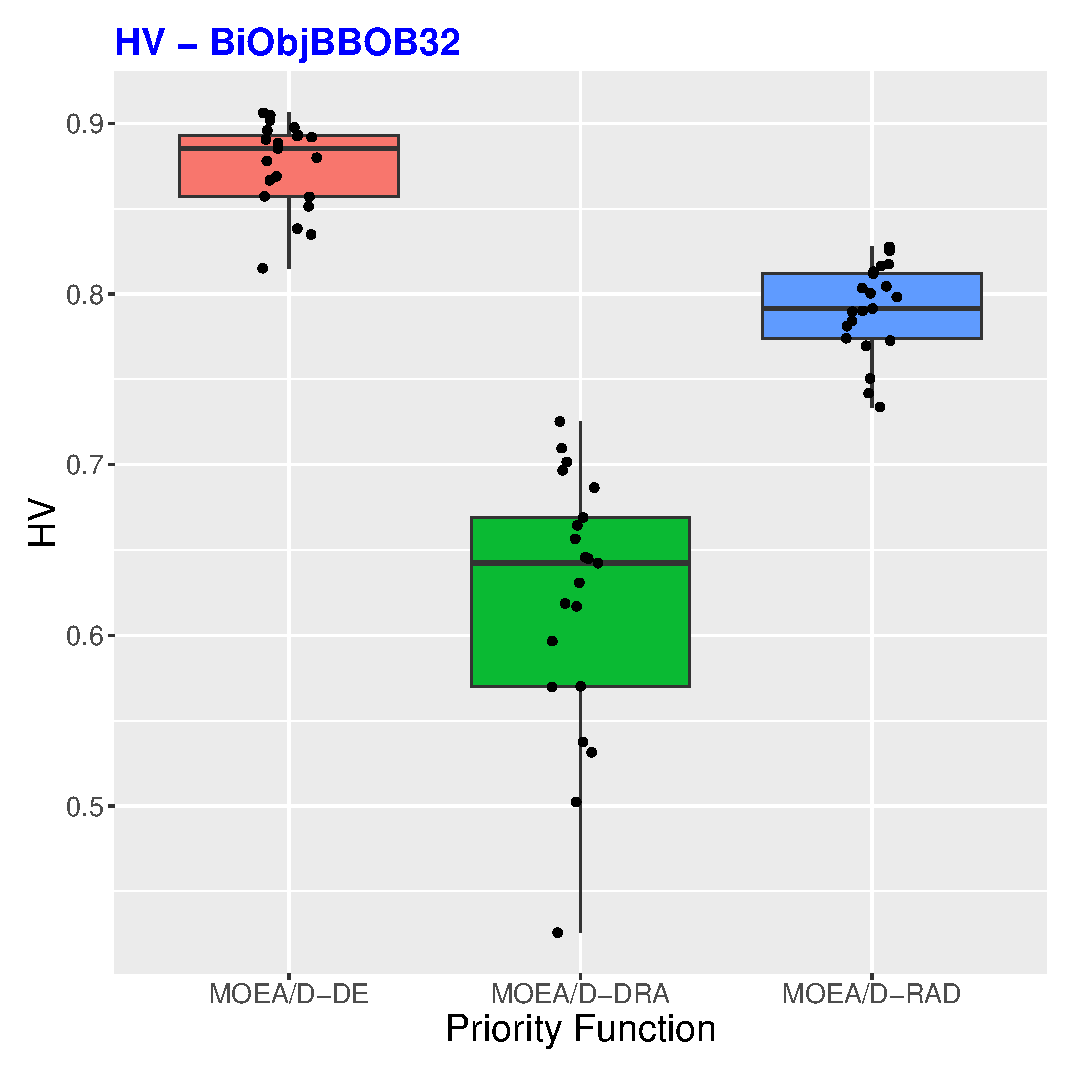
\includegraphics[width=1\textwidth, height=1\textwidth]{img/BiObjBBOB32_HV.eps}
		%	\caption{HV - DTLZ4}
	\end{subfigure}
	\caption{Box plot of HV values on  bbob-biobj-1,  bbob-biobj-26 and  bbob-biobj-32. (Higher values are better)}
	\label{HVS}
\end{figure*}

\begin{figure*}[!t]
	\centering
	%	\Large{Average performance on different tournament size - Gallagher's Gaussian 21-hi Peaks Function}
	\begin{subfigure}[b]{0.33\textwidth}
		\centering
		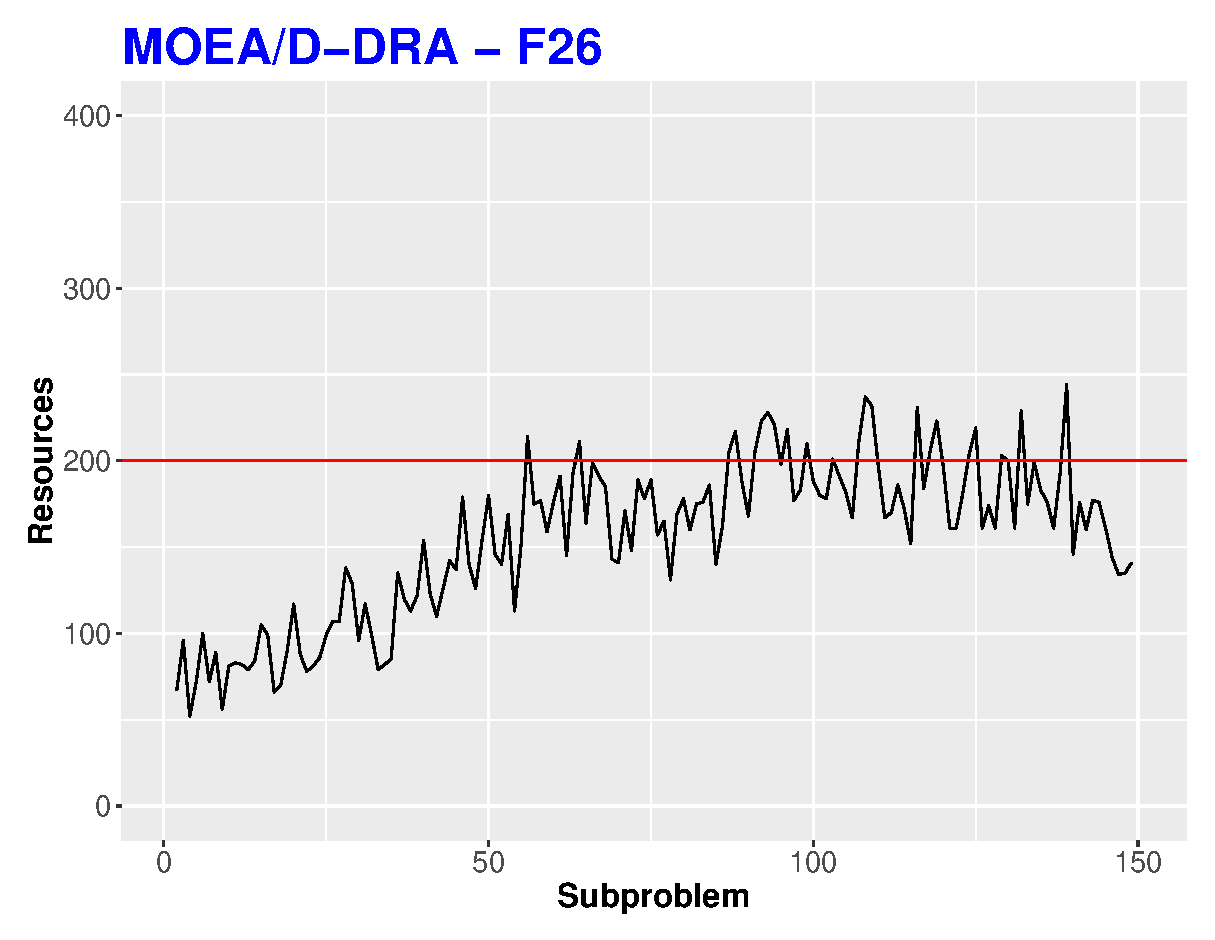
\includegraphics[width=1\textwidth, height=0.8\textwidth]{img/RA-DRA-26.eps}
	\end{subfigure}
	\begin{subfigure}[b]{0.33\textwidth}
		\centering
		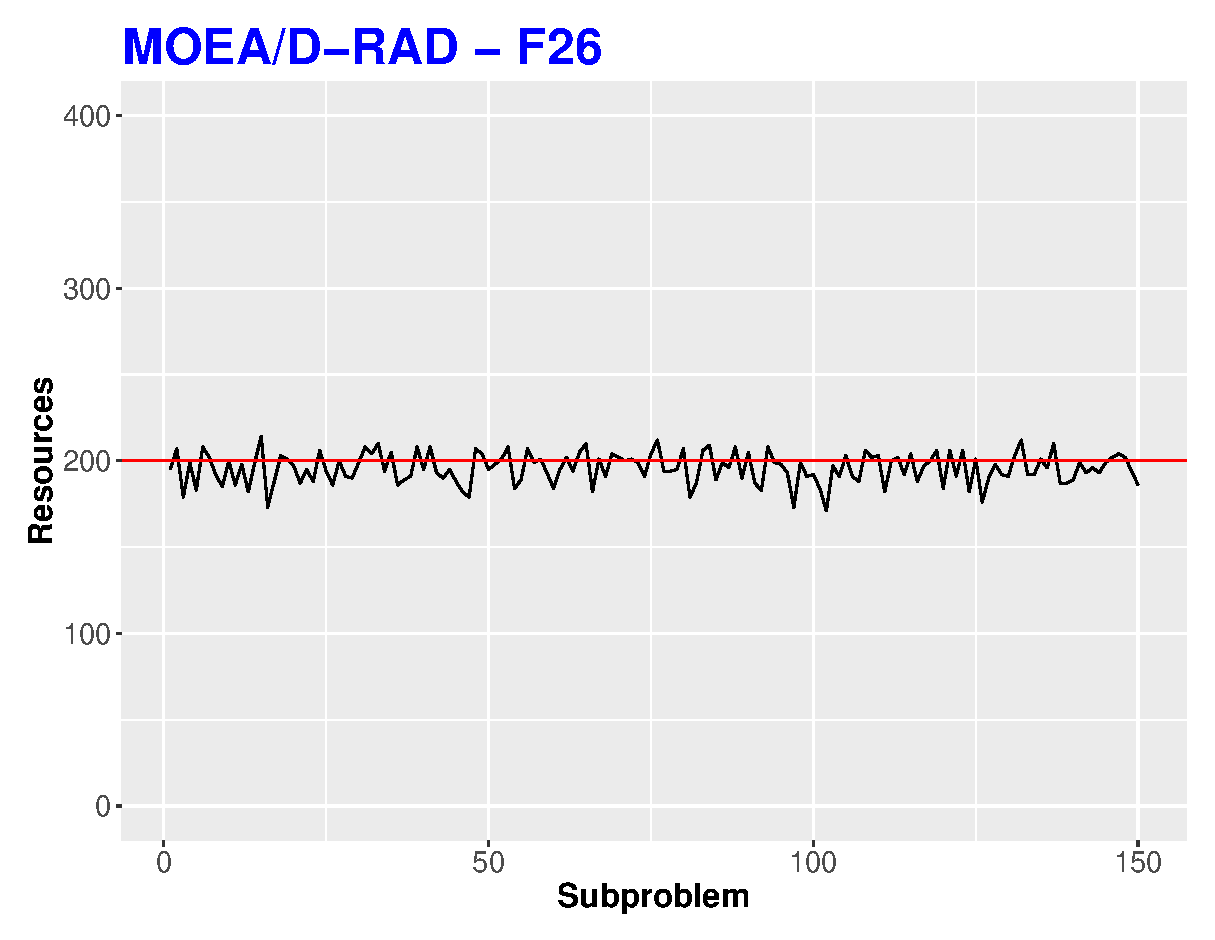
\includegraphics[width=1\textwidth, height=0.8\textwidth]{img/RA-RAD-26.eps}
	\end{subfigure}
	\caption{Resource Allocation by subproblem - The red line indicates the default amount of resource for each problem, i.e., with no priority function.}
	\label{RAs1}
\end{figure*}

\begin{figure*}[!t]
	\centering
	\begin{subfigure}[b]{0.33\textwidth}
		\centering
		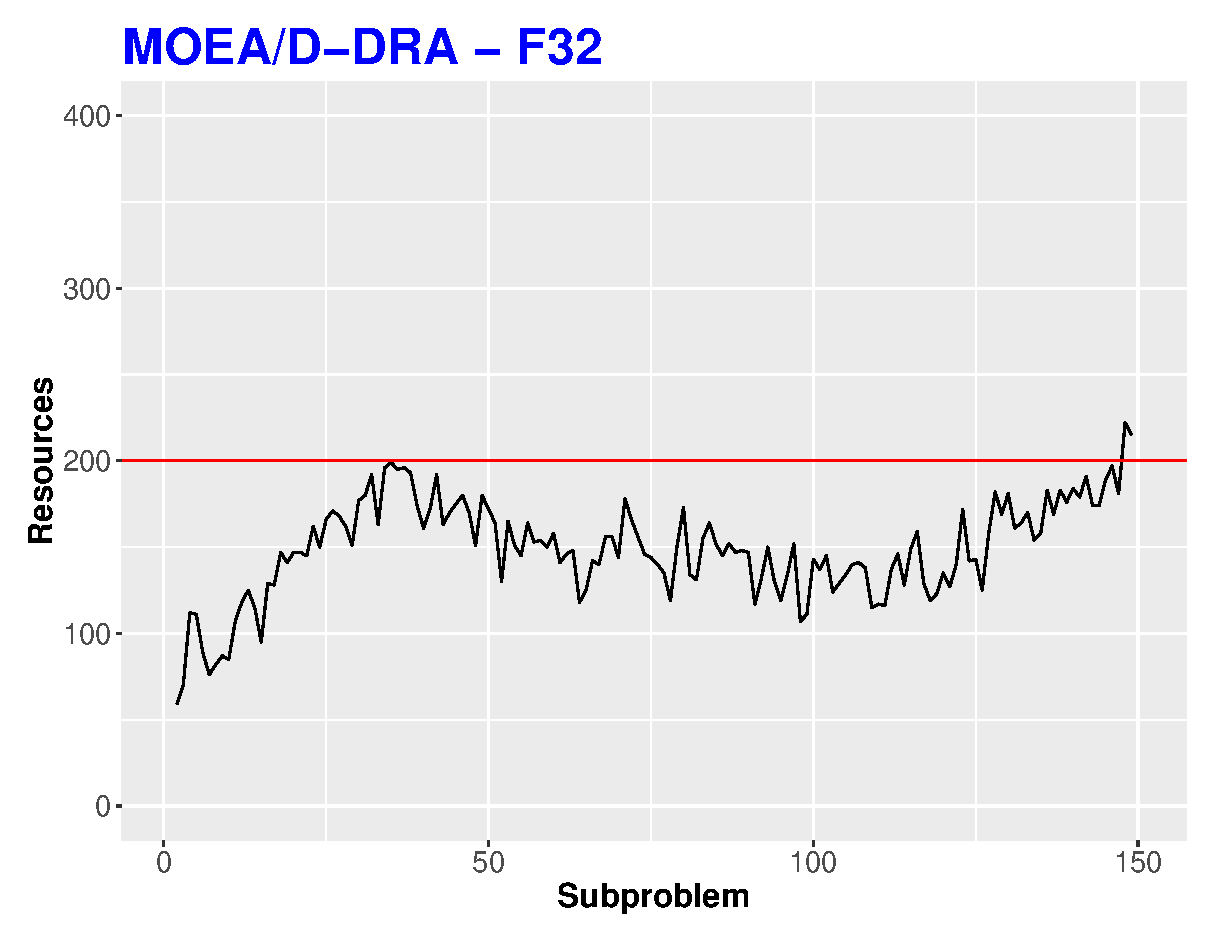
\includegraphics[width=1\textwidth, height=0.8\textwidth]{img/RA-DRA-32.eps}
	\end{subfigure}
	\begin{subfigure}[b]{0.33\textwidth}
		\centering
		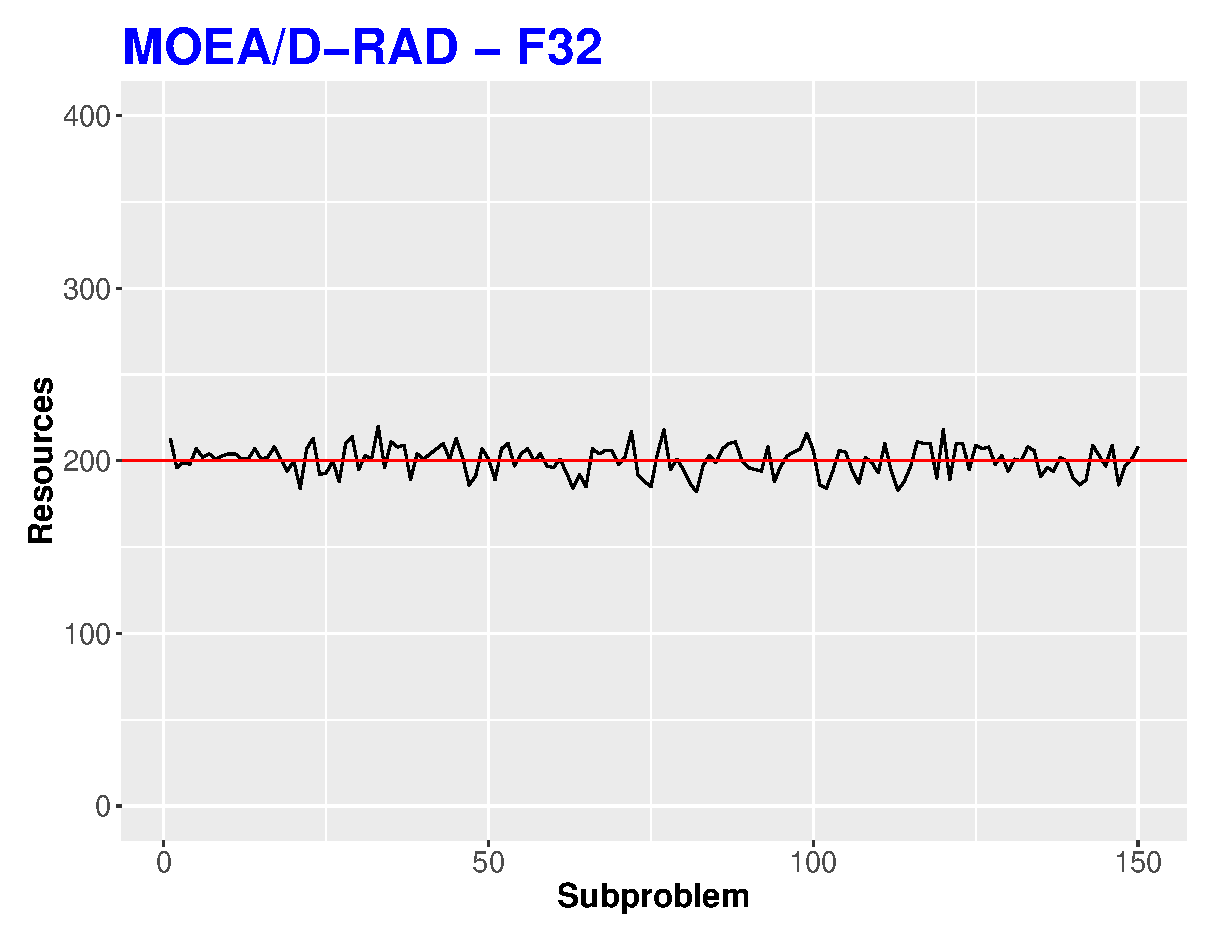
\includegraphics[width=1\textwidth, height=0.8\textwidth]{img/RA-RAD-32.eps}
	\end{subfigure}
	\caption{Resource Allocation by subproblem - The red line indicates the default amount of resource for each problem, i.e., with no priority function.}
	\label{RAs2}
\end{figure*}

\begin{center}

\begin{table*}[!t]
	\tabcolsep=0.33cm
	\footnotesize
	\begin{tabular}{ccccccc}
		\cline{7-7}
		\hline

		\rowcolor[gray]{.5} \multicolumn{1}{|c}{Metric} & \multicolumn{3}{|c|}{HV} &     \multicolumn{3}{c|}{Proportion of Non-dominated} \\ \hline \hline  \hline
		\multicolumn{1}{|l}{Algorithm: }  & \multicolumn{1}{|l|}{MOEA/D-DE} & \multicolumn{1}{l|}{MOEA/D-RAD} & \multicolumn{1}{l|}{MOEA/D-DRA} &  \multicolumn{1}{l|}{MOEA/D-DE} & \multicolumn{1}{l|}{MOEA/D-RAD} & \multicolumn{1}{l|}{MOEA/D-DRA}
		\\ \hline \hline
		\multicolumn{1}{|l|}{Group 1 - F1.}           & \multicolumn{1}{l}{0.8239 (0.005)} & \multicolumn{1}{l}{0.8408 (0.002) } & \multicolumn{1}{l|}{\textbf{0.8519 (0.001)}}
		& \multicolumn{1}{l}{0.460 (0.07)} & \multicolumn{1}{l}{0.910 (0.09) } & \multicolumn{1}{l|}{1.000 (0.00)} \\ \hline
		\multicolumn{1}{|l|}{Group 1 - F2.}              & \multicolumn{1}{l}{0.9480 (0.003)} & \multicolumn{1}{l}{\textbf{0.9572 (0.001)}} & \multicolumn{1}{l|}{0.6435 (0.043)} &		 \multicolumn{1}{l}{0.3933 (0.05)} & \multicolumn{1}{l}{0.800 (0.08) } & \multicolumn{1}{l|}{0.9933 (0.04)} \\ \hline
		 \rowcolor[gray]{.85} \multicolumn{1}{|l|}{Group 2 - F3.}           & \multicolumn{1}{l}{0.9113 (0.002)} & \multicolumn{1}{l}{\textbf{0.9211 (0.001)}} & \multicolumn{1}{l|}{0.5783  (0.043)} & \multicolumn{1}{l}{0.4800 (0.06)} & \multicolumn{1}{l}{0.9133 (0.12)} & \multicolumn{1}{l|}{0.9933 (0.04)}  \\ \hline
		 \rowcolor[gray]{.85} \multicolumn{1}{|l|}{Group 2 - F4.}              & \multicolumn{1}{l}{0.9392 (0.002)} & \multicolumn{1}{l}{\textbf{0.9477 (0.002)}} & \multicolumn{1}{l|}{0.7236 (0.018)}  & \multicolumn{1}{l}{0.4267 (0.06)} & \multicolumn{1}{l}{0.8267 (0.06)} & \multicolumn{1}{l|}{1.0000 (0.01)}  \\ \hline
		\multicolumn{1}{|l|}{Group 3 - F5.}  & \multicolumn{1}{l}{0.6722 (0.008)} & \multicolumn{1}{l}{0.6937 (0.006)} & \multicolumn{1}{l|}{\textbf{0.7024 (0.003)}}  & \multicolumn{1}{l}{0.4867 (0.07)} & \multicolumn{1}{l}{0.9067 (0.07)} & \multicolumn{1}{l|}{1.000 (0.01)}   \\ \hline
		\multicolumn{1}{|l|}{Group 3 - F6.}         & \multicolumn{1}{l}{0.8946 (0.003)} & \multicolumn{1}{l}{0.9092 (0.003)} & \multicolumn{1}{l|}{\textbf{0.9146 (0.002)}}		& \multicolumn{1}{l}{0.4533 (0.05)} & \multicolumn{1}{l}{0.8467 (0.06)} & \multicolumn{1}{l|}{1.000 (0.00)} 		 \\ \hline
		 \multicolumn{1}{|l|}{Group 4 - F7.}  & \multicolumn{1}{l}{0.8313 (0.008)} & \multicolumn{1}{l}{\textbf{0.8350 (0.018)}} & \multicolumn{1}{l|}{0.8173 (0.017)}  & \multicolumn{1}{l}{0.3600 (0.04)} & \multicolumn{1}{l}{0.8533 (0.09)} & \multicolumn{1}{l|}{0.9933 (0.03)}	\\ \hline
		\multicolumn{1}{|l|}{Group 4 -F8.}              & \multicolumn{1}{l}{\textbf{0.8784 (0.016)}} & \multicolumn{1}{l}{0.8159 (0.032)} & \multicolumn{1}{l|}{0.7500 (0.031)} 		& \multicolumn{1}{l}{0.3533 (0.06)} & \multicolumn{1}{l}{0.8533 (0.11)} & \multicolumn{1}{l|}{1.000 (0.02)}  \\ \hline
		\rowcolor[gray]{.85} \multicolumn{1}{|l|}{Group 5 - F9.}           & \multicolumn{1}{l}{0.9526 (0.002)} & \multicolumn{1}{l}{\textbf{0.9583 (0.081)}} & \multicolumn{1}{l|}{0.8340 (0.002)}  		& \multicolumn{1}{l}{0.4533 (0.08)} & \multicolumn{1}{l}{0.867 (0.06)} & \multicolumn{1}{l|}{1.000 (0.04)}  \\ \hline
		\rowcolor[gray]{.85} \multicolumn{1}{|l|}{Group 5 - F10.}              & \multicolumn{1}{l}{0.7780 (0.030)} & \multicolumn{1}{l}{\textbf{0.7882 (0.031)}} & \multicolumn{1}{l|}{0.7484 (0.038)}  		 & \multicolumn{1}{l}{0.5267 (0.07)} & \multicolumn{1}{l}{0.8667 (0.07)} & \multicolumn{1}{l|}{1.000 (0.00)}  \\ \hline
		\multicolumn{1}{|l|}{Group 1 - F11.}           & \multicolumn{1}{l}{0.8214 (0.003)} & \multicolumn{1}{l}{0.8315 (0.001)} & \multicolumn{1}{l|}{\textbf{0.8398 (0.000)}}  	& \multicolumn{1}{l}{0.6000 (0.06)} & \multicolumn{1}{l}{0.9200 (0.05)} & \multicolumn{1}{l|}{1.000 (0.00)}  \\ \hline
		 \rowcolor[gray]{.85} \multicolumn{1}{|l|}{Group 2 - F12.}              & \multicolumn{1}{l}{0.9945 (0.001)} & \multicolumn{1}{l}{\textbf{0.9948 (0.001)}} & \multicolumn{1}{l|}{0.9876 (0.005)}  & \multicolumn{1}{l}{0.4533 (0.08)} & \multicolumn{1}{l}{0.8933 (0.09)} & \multicolumn{1}{l|}{1.000 (0.00)}  \\ \hline
		 \rowcolor[gray]{.85} \multicolumn{1}{|l|}{Group 2 - F13.}           & \multicolumn{1}{l}{0.9890 (0.001)} & \multicolumn{1}{l}{\textbf{0.9907 (0.001)}} & \multicolumn{1}{l|}{0.9855 (0.003)}  	& \multicolumn{1}{l}{0.4200 (0.07)} & \multicolumn{1}{l}{0.8200 (0.11)} & \multicolumn{1}{l|}{1.000 (0.00)}  \\ \hline
		 \multicolumn{1}{|l|}{Group 3 - F14.}              & \multicolumn{1}{l}{0.8995 (0.008)} & \multicolumn{1}{l}{\textbf{0.9155 (0.009)}} & \multicolumn{1}{l|}{0.6580 (0.056)}  		& \multicolumn{1}{l}{0.48733 (0.05)} & \multicolumn{1}{l}{0.8800 (0.08)} & \multicolumn{1}{l|}{0.9933 (0.01)}  \\ \hline
		 \multicolumn{1}{|l|}{Group 3 - F15.}           & \multicolumn{1}{l}{0.9881 (0.002)} & \multicolumn{1}{l}{\textbf{0.9903 (0.002)}} & \multicolumn{1}{l|}{0.8981 (0.033)}  	& \multicolumn{1}{l}{0.3733 (0.06)} & \multicolumn{1}{l}{0.7333 (0.12)} & \multicolumn{1}{l|}{1.000 (0.02)}  \\ \hline
		\multicolumn{1}{|l|}{Group 4 -F16.}              & \multicolumn{1}{l}{\textbf{0.9609 (0.007)}} & \multicolumn{1}{l}{0.9449 (0.009)} & \multicolumn{1}{l|}{0.8562 (0.037)}  		& \multicolumn{1}{l}{0.3533 (0.07)} & \multicolumn{1}{l}{0.8067 (0.09)} & \multicolumn{1}{l|}{0.9867 (0.05)}  \\ \hline
		\multicolumn{1}{|l|}{Group 4 -F17.}           & \multicolumn{1}{l}{\textbf{0.9752 (0.017)}} & \multicolumn{1}{l}{0.9042 (0.022)} & \multicolumn{1}{l|}{0.7901 (0.053)}  	& \multicolumn{1}{l}{0.3000 (0.06)} & \multicolumn{1}{l}{0.7667 (0.11)} & \multicolumn{1}{l|}{0.9733 (0.13)}  \\ \hline
		\rowcolor[gray]{.85} \multicolumn{1}{|l|}{Group 5 - F18.}              & \multicolumn{1}{l}{0.9455 (0.001)} & \multicolumn{1}{l}{\textbf{0.9455 (0.001)}} & \multicolumn{1}{l|}{0.8988 (0.015)}  		& \multicolumn{1}{l}{0.4733 (0.09)} & \multicolumn{1}{l}{0.8533 (0.09)} & \multicolumn{1}{l|}{1.0000 (0.00)}  \\ \hline
		\rowcolor[gray]{.85} \multicolumn{1}{|l|}{Group 5 - F19.}           & \multicolumn{1}{l}{0.9217 (0.025)} & \multicolumn{1}{l}{\textbf{0.9441 (0.057)}} & \multicolumn{1}{l|}{0.6001 (0.182)}  	& \multicolumn{1}{l}{0.4800 (0.09)} & \multicolumn{1}{l}{0.8333 (0.11)} & \multicolumn{1}{l|}{1.000 (0.05)}  \\ \hline
		 \multicolumn{1}{|l|}{Group 6 - F20.}              & \multicolumn{1}{l}{0.9857 (0.001)} & \multicolumn{1}{l}{\textbf{0.9869 (0.001)}} & \multicolumn{1}{l|}{0.9868 (0.001)}  		& \multicolumn{1}{l}{0.5800 (0.09)} & \multicolumn{1}{l}{0.9333 (0.05)} & \multicolumn{1}{l|}{1.0000 (0.00)}  \\ \hline
		\multicolumn{1}{|l|}{Group 6 - F21.}           & \multicolumn{1}{l}{0.9719 (0.001)} & \multicolumn{1}{l}{0.9756 (0.001)} & \multicolumn{1}{l|}{\textbf{0.9766 (0.001)}}  	& \multicolumn{1}{l}{0.4933 (0.07)} & \multicolumn{1}{l}{0.9000 (0.09)} & \multicolumn{1}{l|}{1.000 (0.00)}  \\ \hline
		 \rowcolor[gray]{.85} \multicolumn{1}{|l|}{Group 7 - F22.}              & \multicolumn{1}{l}{0.8035 (0.006)} & \multicolumn{1}{l}{\textbf{0.8177 (0.005)}} & \multicolumn{1}{l|}{0.6182 (0.031)}  		& \multicolumn{1}{l}{0.5067 (0.08)} & \multicolumn{1}{l}{0.8800 (0.06)} & \multicolumn{1}{l|}{1.0000 (0.02)}  \\ \hline
		 \rowcolor[gray]{.85} \multicolumn{1}{|l|}{Group 7 - F23.}           & \multicolumn{1}{l}{0.9677 (0.001)} & \multicolumn{1}{l}{\textbf{0.9714 (0.001)}} & \multicolumn{1}{l|}{0.7871 (0.027)}  	& \multicolumn{1}{l}{0.4933 (0.05)} & \multicolumn{1}{l}{0.8800 (0.08)} & \multicolumn{1}{l|}{0.9933 (0.03)}  \\ \hline
		\multicolumn{1}{|l|}{Group 8 - F24.}              & \multicolumn{1}{l}{\textbf{0.9674 (0.009)}} & \multicolumn{1}{l}{0.9408 (0.013)} & \multicolumn{1}{l|}{0.8609 (0.031)}  		& \multicolumn{1}{l}{0.3933 (0.06)} & \multicolumn{1}{l}{0.7800 (0.11)} & \multicolumn{1}{l|}{0.9800 (0.12)}  \\ \hline
		\multicolumn{1}{|l|}{Group 8 - F25.}           & \multicolumn{1}{l}{\textbf{0.9699 (0.009)}} & \multicolumn{1}{l}{0.9349 (0.012)} & \multicolumn{1}{l|}{0.8647 (0.045)} & \multicolumn{1}{l}{0.3200 (0.05)} & \multicolumn{1}{l}{0.7600 (0.11)} & \multicolumn{1}{l|}{0.9533 (0.13)}  \\ \hline
		 \rowcolor[gray]{.85}  \multicolumn{1}{|l|}{Group 9 - F26.}              & \multicolumn{1}{l}{0.9738 (0.001)} & \multicolumn{1}{l}{\textbf{0.9763 (0.001)}} & \multicolumn{1}{l|}{0.9741 (0.001)}  		& \multicolumn{1}{l}{0.5600 (0.09)} & \multicolumn{1}{l}{0.9467 (0.05)} & \multicolumn{1}{l|}{1.0000 (0.00)}  \\ \hline
		 \rowcolor[gray]{.85} \multicolumn{1}{|l|}{Group 9 - F27.}           & \multicolumn{1}{l}{0.9437 (0.042)} & \multicolumn{1}{l}{\textbf{0.9480 (0.044)}} & \multicolumn{1}{l|}{0.6161 (0.172)} & \multicolumn{1}{l}{0.5467 (0.08)} & \multicolumn{1}{l}{0.8933 (0.06)} & \multicolumn{1}{l|}{0.9867 (0.07)}  \\ \hline
		\multicolumn{1}{|l|}{Group 6 - F28.}              & \multicolumn{1}{l}{0.9808 (0.001)} & \multicolumn{1}{l}{0.9836 (0.001)} & \multicolumn{1}{l|}{\textbf{0.9866 (0.001)}}  		& \multicolumn{1}{l}{0.4067 (0.06)} & \multicolumn{1}{l}{0.8333 (0.09)} & \multicolumn{1}{l|}{1.000 (0.00)}  \\ \hline
		\rowcolor[gray]{.85}  \multicolumn{1}{|l|}{Group 7 - F29.}           & \multicolumn{1}{l}{0.7314 (0.016)} & \multicolumn{1}{l}{\textbf{0.8589 (0.008)}} & \multicolumn{1}{l|}{0.8403 (0.009)} & \multicolumn{1}{l}{0.4600 (0.08)} & \multicolumn{1}{l}{0.8467 (0.07)} & \multicolumn{1}{l|}{1.000 (0.00)}  \\ \hline
		 \rowcolor[gray]{.85} \multicolumn{1}{|l|}{Group 7 - F30.}              & \multicolumn{1}{l}{0.9687 (0.002)} & \multicolumn{1}{l}{\textbf{0.9738 (0.002)}} & \multicolumn{1}{l|}{0.8009 (0.025}  		& \multicolumn{1}{l}{0.4600 (0.06)} & \multicolumn{1}{l}{0.8000 (0.10)} & \multicolumn{1}{l|}{0.9933 (0.03)}  \\ \hline
		\multicolumn{1}{|l|}{Group 8 - F31.}           & \multicolumn{1}{l}{\textbf{0.9255 (0.036)}} & \multicolumn{1}{l}{0.8529 (0.036)} & \multicolumn{1}{l|}{0.7477 (0.045)}		& \multicolumn{1}{l}{0.3400 (0.07)} & \multicolumn{1}{l}{0.8000 (0.08)} & \multicolumn{1}{l|}{0.9733 (0.13)}  \\ \hline
		\multicolumn{1}{|l|}{Group 8 - F32.}              & \multicolumn{1}{l}{\textbf{0.8852 (0.025)}} & \multicolumn{1}{l}{0.7915 (0.026)} & \multicolumn{1}{l|}{0.6423 (0.076)}  		& \multicolumn{1}{l}{0.3400 (0.06)} & \multicolumn{1}{l}{0.7933 (0.07)} & \multicolumn{1}{l|}{0.9733 (0.12)}  \\ \hline
		\rowcolor[gray]{.85} \multicolumn{1}{|l|}{Group 9 - F33.}  & \multicolumn{1}{l}{0.9849 (0.001)} & \multicolumn{1}{l}{0.9867 (0.000)} & \multicolumn{1}{l|}{\textbf{0.9885 (0.031)}}  		& \multicolumn{1}{l}{0.4400 (0.05)} & \multicolumn{1}{l}{0.7867 (0.08)} & \multicolumn{1}{l|}{1.0000 (0.00)} \\ \hline
		 \rowcolor[gray]{.85} \multicolumn{1}{|l|}{Group 9 - F34.}              & \multicolumn{1}{l}{0.8744 (0.038)} & \multicolumn{1}{l}{\textbf{0.8776 (0.031)}} & \multicolumn{1}{l|}{0.6388 (0.182)}  		& \multicolumn{1}{l}{0.5000 (0.11)} & \multicolumn{1}{l}{0.8400 (0.10)} & \multicolumn{1}{l|}{1.0000 (0.01)}  \\ \hline
		\multicolumn{1}{|l|}{Group 10 - F35.}  & \multicolumn{1}{l}{0.5550 (0.003} & \multicolumn{1}{l}{0.5831 (0.004)} & \multicolumn{1}{l|}{\textbf{0.5956 (0.003)}}  		& \multicolumn{1}{l}{0.5067 (0.07)} & \multicolumn{1}{l}{0.9000 (0.07)} & \multicolumn{1}{l|}{01.000 (0.00)} \\ \hline
		  \multicolumn{1}{|l|}{Group 10 - F36.}              & \multicolumn{1}{l}{0.7872 (0.006)} & \multicolumn{1}{l}{\textbf{0.7983 (0.006)}} & \multicolumn{1}{l|}{0.7872 (0.006)}  		& \multicolumn{1}{l}{0.4733 (0.08)} & \multicolumn{1}{l}{0.8733 (0.09)} & \multicolumn{1}{l|}{0.9933 (0.01)}  \\ \hline
		\multicolumn{1}{|l|}{Group 11 - F37.}  & \multicolumn{1}{l}{0.7367 (0.009)} & \multicolumn{1}{l}{0.7425 (0.010)} & \multicolumn{1}{l|}{\textbf{0.7479 (0.013)}}  		& \multicolumn{1}{l}{0.4000 (0.05)} & \multicolumn{1}{l}{0.8667 (0.08)} & \multicolumn{1}{l|}{1.000 (0.01)} \\ \hline
		\multicolumn{1}{|l|}{Group 11 - F38.}              & \multicolumn{1}{l}{\textbf{0.8619 (0.010)}} & \multicolumn{1}{l}{0.8550 (0.011)} & \multicolumn{1}{l|}{0.8461 (0.019)}  		& \multicolumn{1}{l}{0.3133 (0.05)} & \multicolumn{1}{l}{0.8667 (0.07)} & \multicolumn{1}{l|}{0.9867 (0.04)}  \\ \hline
		\rowcolor[gray]{.85}  \multicolumn{1}{|l|}{Group 12 - F39.}  & \multicolumn{1}{l}{0.8128 (0.005)} & \multicolumn{1}{l}{\textbf{0.8285 (0.004)}} & \multicolumn{1}{l|}{0.7280 (0.015)}  		& \multicolumn{1}{l}{0.5067 (0.08)} & \multicolumn{1}{l}{0.9000 (0.07)} & \multicolumn{1}{l|}{1.0000 (0.00)} \\
		\hline
		\rowcolor[gray]{.85}  \multicolumn{1}{|l|}{Group 12 - F40.}              & \multicolumn{1}{l}{0.4736 (0.047)} & \multicolumn{1}{l}{\textbf{0.5116 (0.048)}} & \multicolumn{1}{l|}{0.3954 (0.042)}  		& \multicolumn{1}{l}{0.6333 (0.08)} & \multicolumn{1}{l}{0.9467 (0.03)} & \multicolumn{1}{l|}{1.0000 (0.01)}  \\ \hline
		\multicolumn{1}{|l|}{Group 10 - F41.}  & \multicolumn{1}{l}{0.9281 (0.0.003)} & \multicolumn{1}{l}{0.9368 (0.004)} & \multicolumn{1}{l|}{\textbf{0.9480 (0.003)}}  		& \multicolumn{1}{l}{0.4133 (0.06)} & \multicolumn{1}{l}{0.8267 (0.10)} & \multicolumn{1}{l|}{1.0000 (0.00} \\ \hline
		\multicolumn{1}{|l|}{Group 11 - F42.}              & \multicolumn{1}{l}{\textbf{0.9379 (0.010)}} & \multicolumn{1}{l}{0.9034 (0.021)} & \multicolumn{1}{l|}{0.8975 (0.021)}  		& \multicolumn{1}{l}{0.3667 (0.06)} & \multicolumn{1}{l}{0.8467 (0.08)} & \multicolumn{1}{l|}{0.9933 (0.03)}  \\ \hline
		\multicolumn{1}{|l|}{Group 11 - F43.}  & \multicolumn{1}{l}{\textbf{0.8744 (0.026)}} & \multicolumn{1}{l}{0.7937 (0.031)} & \multicolumn{1}{l|}{0.7410 (0.060)}  		& \multicolumn{1}{l}{0.3733 (0.07)} & \multicolumn{1}{l}{0.7800 (0.10)} & \multicolumn{1}{l|}{0.9533 (0.15} \\ \hline
		\rowcolor[gray]{.85}  \multicolumn{1}{|l|}{Group 12 - F44.}              & \multicolumn{1}{l}{0.9687 (0.003)} & \multicolumn{1}{l}{\textbf{0.9761 (0.002}} & \multicolumn{1}{l|}{0.9032 (0.011)}  		& \multicolumn{1}{l}{0.4067 (0.06)} & \multicolumn{1}{l}{0.8200 (0.08)} & \multicolumn{1}{l|}{0.9867 (0.04)} \\ \hline
		\rowcolor[gray]{.85} \multicolumn{1}{|l|}{Group 12 - F45.}  & \multicolumn{1}{l}{0.8091 (0.043)} & \multicolumn{1}{l}{0.8223 (0.052)} & \multicolumn{1}{l|}{\textbf{0.8557 (0.063)}}  		& \multicolumn{1}{l}{0.5200 (0.07)} & \multicolumn{1}{l}{0.8867 (0.05)} & \multicolumn{1}{l|}{1.0000 (0.01} \\ \hline
		\multicolumn{1}{|l|}{Group 13 - F46.}              & \multicolumn{1}{l}{\textbf{0.8817 (0.012)}} & \multicolumn{1}{l}{0.8428 (0.023} & \multicolumn{1}{l|}{0.8378 (0.027)}  		& \multicolumn{1}{l}{0.2933 (0.06)} & \multicolumn{1}{l}{0.8467 (0.09)} & \multicolumn{1}{l|}{1.000 (0.03)}  \\ \hline
		\multicolumn{1}{|l|}{Group 13 - F47.}  & \multicolumn{1}{l}{\textbf{0.8208 (0.031)}} & \multicolumn{1}{l}{0.6803 (0.043)} & \multicolumn{1}{l|}{0.5553 (0.071)}  		& \multicolumn{1}{l}{0.4000 (0.08)} & \multicolumn{1}{l}{0.8667 (0.08)} & \multicolumn{1}{l|}{0.9933 (0.04} \\ \hline
		\multicolumn{1}{|l|}{Group 14 - F48.} & \multicolumn{1}{l}{\textbf{0.9520 (0.0018)}} & \multicolumn{1}{l}{0.8673 (0.033)} & \multicolumn{1}{l|}{0.7799 (0.044)} & \multicolumn{1}{l}{0.3400 (0.07)} & \multicolumn{1}{l}{0.7067 (0.13)} & \multicolumn{1}{l|}{0.9733 (0.17)}  \\ \hline
		\multicolumn{1}{|l|}{Group 14 - F49.}  & \multicolumn{1}{l}{\textbf{0.8967 (0.051)}} & \multicolumn{1}{l}{0.8730 (0.059)} & \multicolumn{1}{l|}{0.8579 (0.068)}  		& \multicolumn{1}{l}{0.4533 (0.07)} & \multicolumn{1}{l}{0.8533 (0.07)} & \multicolumn{1}{l|}{1.000 (0.03} \\ \hline
		\multicolumn{1}{|l|}{Group 13 - F50.}              & \multicolumn{1}{l}{\textbf{0.8794 (0.036)}} & \multicolumn{1}{l}{0.7626 (0.038)} & \multicolumn{1}{l|}{0.7402 (0.031)}  		& \multicolumn{1}{l}{0.3667 (0.07)} & \multicolumn{1}{l}{0.8600 (0.07)} & \multicolumn{1}{l|}{1.000 (0.01)}  \\ \hline% \hline \hline
		\multicolumn{1}{|l|}{Group 14 - F51.}  & \multicolumn{1}{l}{\textbf{0.9801 (0.008)}} & \multicolumn{1}{l}{0.9535 (0.009)} & \multicolumn{1}{l|}{0.9218 (0.017)}  		& \multicolumn{1}{l}{0.3467 (0.06)} & \multicolumn{1}{l}{0.8000 (0.11)} & \multicolumn{1}{l|}{0.9667 (0.20} \\ \hline
		\multicolumn{1}{|l|}{Group 14 - F52.}              & \multicolumn{1}{l}{\textbf{0.8839 (0.060)}} & \multicolumn{1}{l}{0.8652 (0.069)} & \multicolumn{1}{l|}{0.8414 (0.074)}  		& \multicolumn{1}{l}{0.4067 (0.07)} & \multicolumn{1}{l}{0.8533 (0.10)} & \multicolumn{1}{l|}{1.0000 (0.109)}  \\ \hline % \hline \hline
		\multicolumn{1}{|l|}{Group 15 - F53.}  & \multicolumn{1}{l}{0.9927 (0.000)} & \multicolumn{1}{l}{0.9929 (0.000)} & \multicolumn{1}{l|}{\textbf{0.9930 (0.00)}}  		& \multicolumn{1}{l}{0.5267 (0.05)} & \multicolumn{1}{l}{0.8600 (0.06)} & \multicolumn{1}{l|}{1.0000 (0.00} \\ \hline
		\multicolumn{1}{|l|}{Group 15 - F54.}              & \multicolumn{1}{l}{\textbf{0.8950 (0.045)}} & \multicolumn{1}{l}{0.8717 (0.057)} & \multicolumn{1}{l|}{0.7629 (0.135)}  		& \multicolumn{1}{l}{0.5267 (0.08)} & \multicolumn{1}{l}{0.9000 (0.07)} & \multicolumn{1}{l|}{1.000 (0.02)}  \\ \hline
		\multicolumn{1}{|l|}{Group 15 - F55.}  & \multicolumn{1}{l}{\textbf{0.3855 (0.070)}} & \multicolumn{1}{l}{0.3769 (0.084)} & \multicolumn{1}{l|}{0.3709 (0.111)}  		& \multicolumn{1}{l}{0.8867 (0.07)} & \multicolumn{1}{l}{0.9733 (0.02)} & \multicolumn{1}{l|}{1.000 (0.00} \\ \hline \hline \hline
	\end{tabular}
	\caption{On the left side, HV medians and standard deviations, in parenthesis for every function/priority function. The best values found by a priority function are in bold. On the right side, mean of the percentage of the median values and mean of the median values of the standard deviation (in parenthesis) of non-dominated solutions for every function/priority function. Shaded lines show the groups MOEA/D-RAD was specially successfulin terms of hypervolume values.}
	\label{stats}
\end{table*}
\end{center}

\begin{table}[!t]
	\begin{tabular}{lll}
		\hline
		\rowcolor[gray]{.7} \multicolumn{1}{|l|}{\textbf{HV}}  & \multicolumn{1}{|l|}{MOEA/D-DRA} & \multicolumn{1}{l|}{MOEA/D-RAD} \\ \hline \hline \hline
		MOEA/D-RAD                      &  3.1e-08                      & -                                      \\
		\rowcolor[gray]{.95} MOEA/D-DE                      &  3.1e-08                   &  3.1e-08                 \\
	\end{tabular}
	\caption{Statistical Analysis of the HV results based on the Pairwise Wilcoxon Rank Sum Test. It shows that exists significant difference between the ranks of MOEA/D-RAD, MOEA/D-DRA and MOEA/D-DE.}
	\label{statistics}
\end{table}

\ref{HVS} shows the boxplots of the hypervolume values obtained by the three methods
on functions F26, F1 and F32 of bbob-biobj. F26 is an example of a moderate and
weakly structured function (group 9), where MOEA/D-RAD performed best. F1  is a
separable and separable function (group 1), where MOEA/D-DRA performed best, and
F32 is a moderate and multi-modal function (group 8), where MOEA/D-DE performed
.

\ref{stats} gives us a general view of these results over all functions and
function groups. In general, MOEA/D-RAD performed better than the other methods
(or second best) in terms of hypervolume. This ranking is reinforced by a
Pairwise Wilcoxon Rank Test over the entire experiment~(\ref{statistics}).

However, a post-hoc analysis of these results focusing on the function groups
suggests some interesting properties of the three methods. We observe that
MOEA/D-RAD was specially successful for function groups that included
moderate-conditioned or weakly-structured functions (groups 2, 5, 6, 7, 8, 9, 12 and
15, shaded in \ref{stats}), and performed slightly worse for groups including
multi-modal functions (groups 4, 8, 11, 13 and 14). In particular, we find it  very
interesting that MOEA/D-DE without priority performed better in the multi-modal
groups. This post-hoc analysis suggests a follow up experiment to confirm this
observations.

\subsection{Proportion of Non-dominated Solutions}

Another difference that we see among the algorithms  is the proportion of non
dominated solutions. The results on the~\ref{stats} indicate that MOEA/D-DRA
leads to the highest rate of non-dominated solutions in the final solution set,
followed by MOEA/D-RAD. In general, both substantially improve this proportion
over the results of MOEA/D-DE.  It seems that there is no relation between
hypervolume performance and the proportion of non-dominated solutions.


\subsection{Resource Allocation}


\ref{RAs1} and \ref{RAs2} illustrate the amount resource allocated by MOEA/D-DRA
and MOEA/D-RAD to each subproblem on problems F26 and F32. MOEA/D-DE is
not included since it does not perform resource allocation.

These figures show how the choice of priority function influences the
resource allocation. The resource allocation by MOEA/D-DRA is much more
adaptive to each problem, while the resource allocation done by
MOEA/D-RAD is more conservative and uniform.

However, even though the resource allocation behavior seen in these figures
may seem limited, it is clear from \ref{stats} that it has a deep impact on
the performance of the algorithm.

\section{Conclusion}

In this research, we propose a new algorithm for Resource Allocation in Multi-Objective Optimization, MOEA/D-RAD. The performance of this algorithm is studied on the bbob-biobj. benchmark functions. This algorithm differs from the standard MOEA/D by using Resource Allocation techniques computational effort proportional to each subproblem's difficulty. 

MOEA/D-RAD uses a priority function based on a geometrical perspective, MRDL, for Resource Allocation. This algorithm determines the computational resource assigned to each subproblem, based on its contribution to the overall diversity of the population.

We have compared the new approach with the MOEA/D-DE and a variant with dynamic resource allocation strategy, MOEA/D-DRA, and the experimental results suggested our method performs well on many test problems.

MOEA/D-RAD showed a better performance on bbob-biobj, specially in functions that are in the  moderate-conditioned and weakly-structured groups. Although MOEA/D-DRA lead to the highest rate of non-dominated solutions in the final solution set, MOEA/D-RAD could be seem as an improvement to the MOEA/D-DE proportion values.

Since the Resource Allocation distribution of MOEA/D-RAD is not so much different to the one of MOEA/D-DE we understand that this explains why the results in the hypervolume metric of the MOEA/D-RAD tend to be better, but not so much different to the hypervolume values of the MOEA/D-DE. Consequently, we conclude that MOEA/D-RAD does represent a improvement in diversity not only since it improves the hypervolume metrics in many functions but since for \textit{all} functions the proportion of non-dominated solutions is always higher.

Overall, the findings of this work strengthens the idea that Resource Allocation techniques are worth of attention, specially those that focuses on critical issues (such as diversity in the object space). This suggests the choice of priority functions is a critical component of a Resource Allocation system. Our results indicate that MOEA/D-RAD might be a  reasonable choices MOP where at least one objective is in one of the following groups: moderate-conditioned; and weakly-structured. It is crucial to  explore this further.


In this work, we do not yet consider archive based Resource Allocation and archive based priority functions, such as MOEA/D-CRA~\cite{kang2018collaborative}. We will address this issue in a continuation to this study. There are many components and variants of MOEA/D and is interesting to combine the Norm priority function with the them. Then, we can further explore the relationship of priority functions based on diversity with others components and variants of the MOEA/D framework. How to define more efficient and effective utility functions for different problems is also worth further investigation (such as priority function that also consider constraints) as well as to verify the results of using priority function in other real-world problems.
%

\bibliography{sample}
\bibliographystyle{jpnsec}

%\bibliographystyle{IEEEtran}

%\bibliography{sample}
%\bibliographystyle{jpnsec}

%
%􏰂
%
%\begin{biography}
%\profile{m}{進化 太郎}{著者の略歴}{portrait}
%\end{biography}


%\appendix
%\section{Appendix}
%
%%% Biography %%%%%%%%%%%%%%%%%%%%%%%%%%%%%%%%%%%%%%%%%%%%%%%%%%%%%%%%%%%%%%%%%%


\end{document}
